\documentclass[11pt]{article}

\usepackage[letterpaper,margin=1in]{geometry}
\usepackage[T1]{fontenc}
\usepackage[utf8]{inputenc}
\usepackage{lmodern}
\usepackage{microtype}
\usepackage{graphicx}
\usepackage{booktabs}
\usepackage{array}
\usepackage{enumitem}
\usepackage{caption}
\usepackage{subcaption}
\usepackage{placeins}
\usepackage{xcolor}
\usepackage{xurl}
\usepackage{hyperref}
\usepackage{titlesec}
\usepackage{fancyhdr}

\graphicspath{{report_assets/}{report_assets/original_unique/}}

\definecolor{linkblue}{RGB}{20, 86, 150}
\definecolor{darkgray}{RGB}{45, 45, 45}

\hypersetup{
  colorlinks=true,
  linkcolor=linkblue,
  urlcolor=linkblue,
  citecolor=linkblue,
  pdftitle={Quest 3 Bowling Training Aid Technical Report},
  pdfauthor={Cale Rudolph, Srinivas Kantha Reddy, Apurv Kushwaha}
}

\setlist[itemize]{leftmargin=1.3em,itemsep=0.25em,topsep=0.25em}
\setlist[enumerate]{leftmargin=1.6em,itemsep=0.25em,topsep=0.25em}
\captionsetup{font=small,labelfont=bf}
\Urlmuskip=0mu plus 1mu
\emergencystretch=2em
\newcommand{\codepath}[1]{\path{#1}}
\newcommand{\reportlink}[2]{\href{#1}{\textcolor{linkblue}{#2}}}
\titleformat{\section}{\Large\bfseries\color{darkgray}}{\thesection}{0.7em}{}
\titleformat{\subsection}{\large\bfseries\color{darkgray}}{\thesubsection}{0.7em}{}
\titlespacing*{\section}{0pt}{1.4em}{0.6em}
\titlespacing*{\subsection}{0pt}{1.0em}{0.4em}

\pagestyle{fancy}
\fancyhf{}
\lhead{\small Quest 3 Bowling Training Aid}
\rhead{\small CSCI 5629 Course Project}
\cfoot{\thepage}
\renewcommand{\headrulewidth}{0.4pt}

\begin{document}
\pagenumbering{Roman}

\begin{titlepage}
  \centering
  \vspace*{1.25in}

  {\Huge\bfseries Quest 3 Bowling Training Aid\par}
  \vspace{0.25in}
  {\Large Technical Project Report\par}

  \vspace{0.55in}
  {\large CSCI 5629 Course Project\par}
  \vspace{0.12in}
  {\large May 2026\par}

  \vspace{0.55in}
  {\large Cale Rudolph\par}
  \vspace{0.08in}
  {\large Srinivas Kantha Reddy\par}
  \vspace{0.08in}
  {\large Apurv Kushwaha\par}

  \vspace{0.75in}
  \begin{minipage}{0.68\textwidth}
    \centering
    \normalsize\itshape
    Live lane-anchored replay with YOLO, SAM2, and mixed-reality feedback for real bowling sessions.
  \end{minipage}

  \vfill
  {\small Project links are listed in the References section.}
\end{titlepage}

\clearpage
\pagenumbering{arabic}

\begin{abstract}
Quest 3 Bowling Training Aid is a mixed-reality bowling replay prototype for Meta Quest 3 and a Windows laptop. The headset captures passthrough camera video from a real bowling lane, encodes it as H.264, sends frame metadata and lane calibration information to the laptop, and receives shot results back from the laptop. The laptop detects a bowling ball with a dedicated YOLO26s detector, initializes SAM2 camera tracking from that seed, reconstructs the ball path in lane coordinates, computes bowling-specific statistics, and publishes replay results. The headset then renders the result as a lane-anchored trajectory replay with shot statistics and a session review interface.

The main contribution of the project is not any single detector or overlay. The key contribution is a working end-to-end loop: physical lane calibration, live capture, robust networking, model inference, geometric reconstruction, result validation, and mixed-reality feedback. The final prototype demonstrates that an ordinary bowling alley can be augmented with immediate coaching feedback using a consumer headset and a laptop, while still being honest about the limitations of camera-based tracking near the pin deck.
\end{abstract}

\begin{figure}[ht]
  \centering
  \begin{subfigure}{0.48\textwidth}
    \centering
    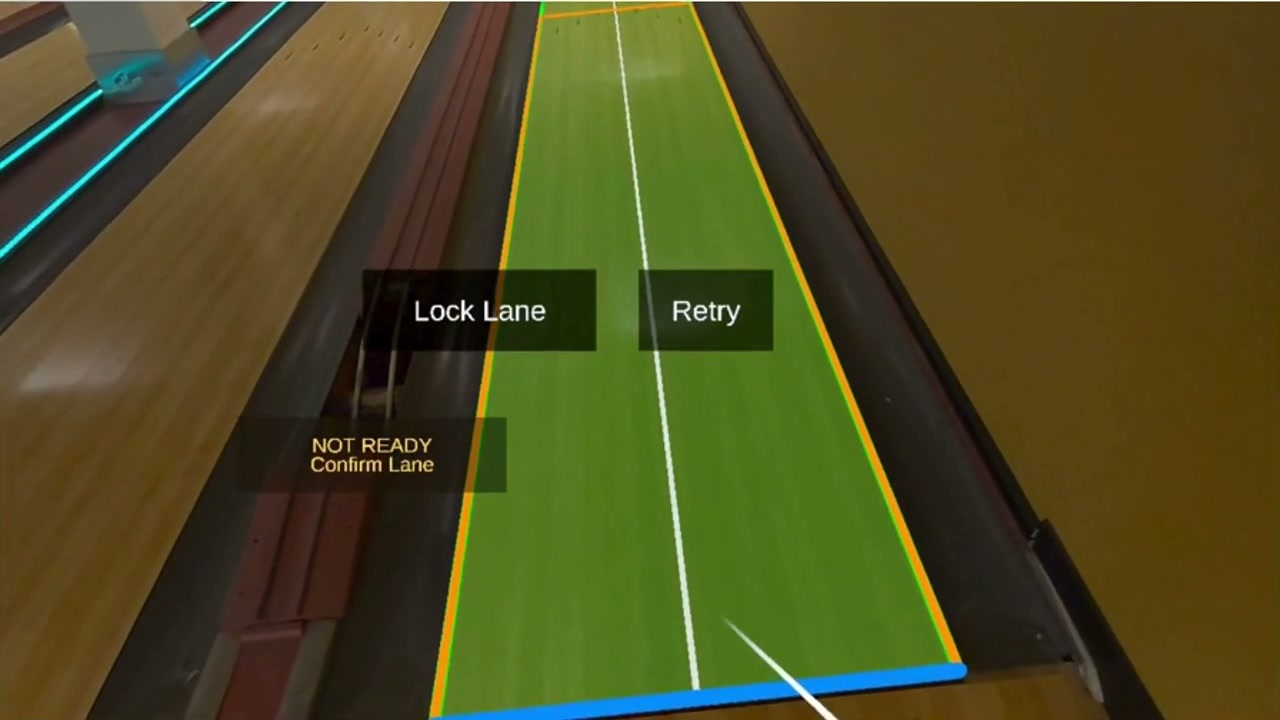
\includegraphics[width=\linewidth]{selected_stills_clean/fig1a_lane_confirmation.jpg}
    \caption{Calibrate: align and confirm the lane.}
  \end{subfigure}
  \hfill
  \begin{subfigure}{0.48\textwidth}
    \centering
    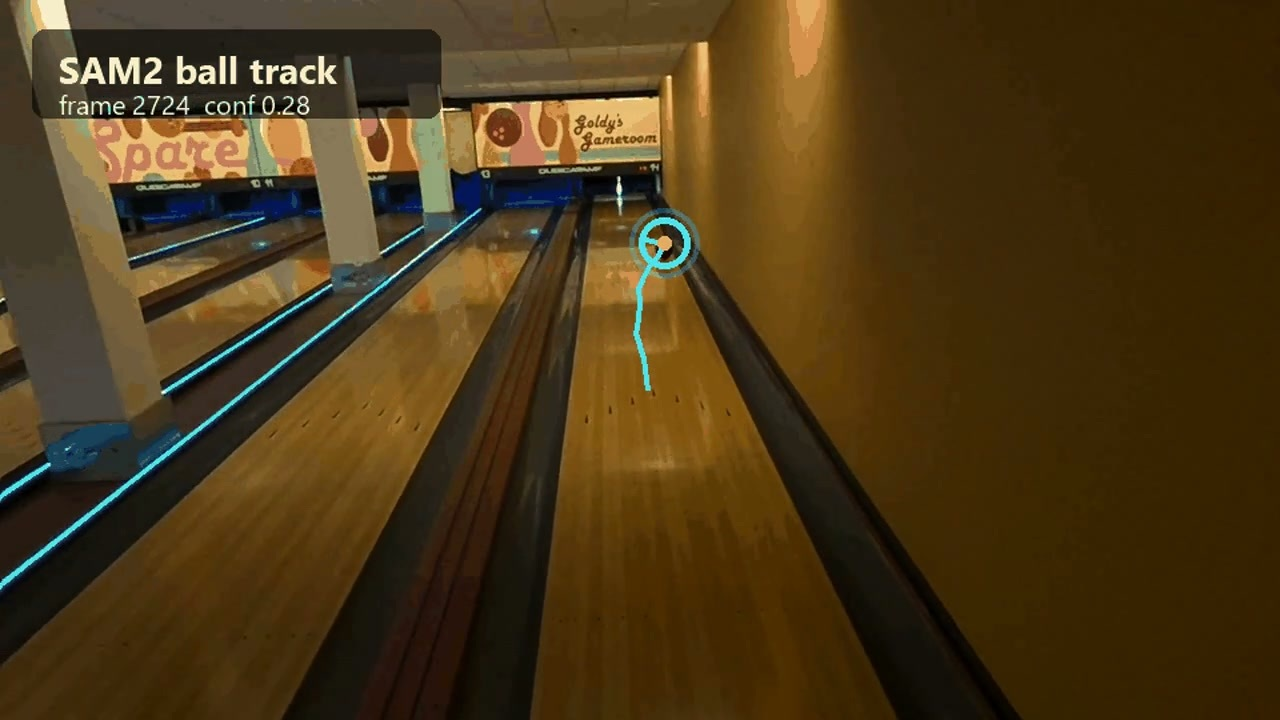
\includegraphics[width=\linewidth]{selected_stills_clean/fig1d_sam2_tracking.jpg}
    \caption{Track: follow the ball with SAM2.}
  \end{subfigure}

  \vspace{0.6em}
  \begin{subfigure}{0.48\textwidth}
    \centering
    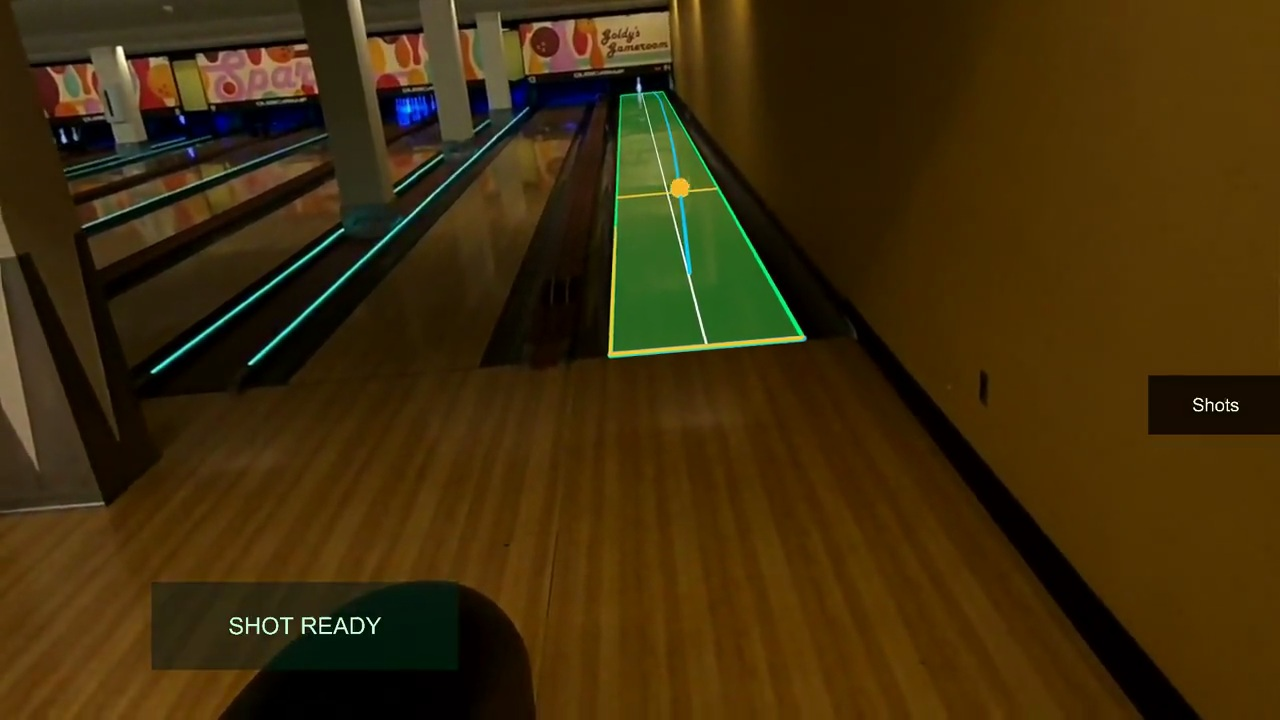
\includegraphics[width=\linewidth]{selected_stills_clean/fig1b_replay_view.jpg}
    \caption{Replay: render the path on the lane.}
  \end{subfigure}
  \hfill
  \begin{subfigure}{0.48\textwidth}
    \centering
    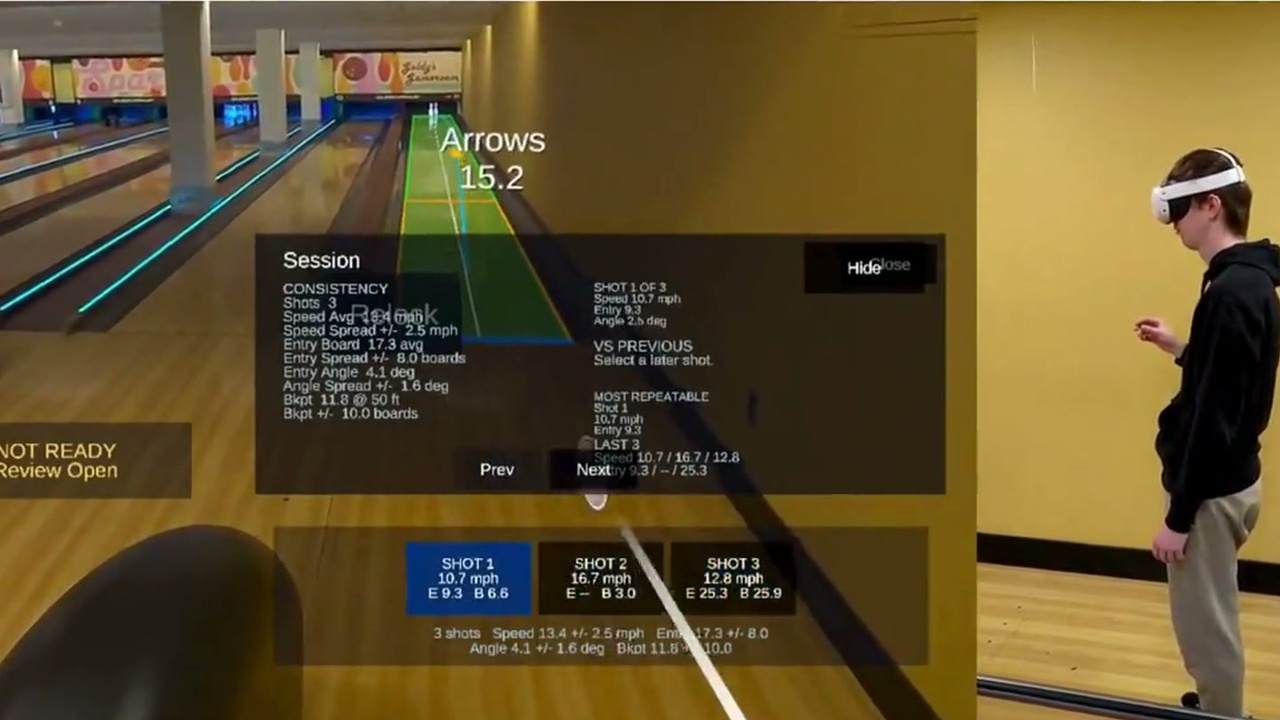
\includegraphics[width=\linewidth]{selected_stills_clean/fig1c_session_review.jpg}
    \caption{Review: compare shots and stats.}
  \end{subfigure}
  \caption{Overview of the end-to-end experience, read left-to-right and top-to-bottom: calibrate the lane, track the ball, replay the trajectory, and review the session.}
\end{figure}
\FloatBarrier

\section{Motivation and Goal}

Bowling scoreboards tell a bowler which pins fell, but they do not explain the path of the ball. A bowler often wants to know where the ball crossed the arrows, where it broke, how much speed it lost, and whether it entered the pocket on the intended board. These are the kinds of details that professional coaching systems and instrumented lanes can provide, but most recreational bowlers do not have access to that equipment. Phone video helps somewhat, but it is usually delayed, manually reviewed, and not transformed into lane-space measurements.

Our motivation was to build a portable mixed-reality training aid that could sit on top of a normal bowling session. The intended users are bowlers who want quick feedback after each throw, coaches who want a portable replay tool, and students or developers interested in live sports analytics with wearable cameras. In the ideal user experience, the bowler puts on the Quest, aligns a virtual lane with the real lane, waits for a clear \emph{Shot Ready} state, throws the ball, and sees the reconstructed path appear on the physical lane in the headset.

The expected features were:
\begin{itemize}
  \item headset-side lane placement and confirmation;
  \item live H.264 passthrough streaming from Quest to laptop;
  \item per-frame metadata with camera pose, intrinsics, timestamps, and lane events;
  \item YOLO-based causal ball discovery;
  \item SAM2 mask tracking from the YOLO seed;
  \item lane-space trajectory reconstruction and smoothing;
  \item speed, board, breakpoint, and entry statistics;
  \item in-headset replay, shot list, and session review;
  \item explicit \emph{Shot Ready} and \emph{Shot Not Ready} states so the bowler knows when the system can be trusted.
\end{itemize}

The final design goal was trust. A visually convincing line drawn on the lane is not useful if it is spatially wrong or attached to stale calibration. Therefore the final code treats the Quest-confirmed lane as the source of truth, validates shot results against the current lane lock, and blocks the throw view until media, metadata, results, lane lock, and laptop pipeline state are all synchronized.

\section{System Overview and User Flow}

The final system is split into a Quest runtime and a laptop runtime. The Quest side handles mixed-reality interaction, lane placement, GPU frame capture, Android H.264 encoding, and replay rendering. The laptop side handles receiving and persisting live streams, decoding frames, running YOLO and SAM2, reconstructing trajectory points, computing statistics, and publishing structured results back to the headset.

The live user flow is:
\begin{enumerate}
  \item The laptop pipeline starts and advertises itself over UDP discovery.
  \item The Quest app connects media, metadata, and result channels.
  \item The bowler pinch-and-holds the lane overlay, aligns it with the real foul line/lane, releases to preview, and confirms the lane.
  \item Quest sends a lane confirmation containing the complete lane geometry.
  \item The laptop arms shot detection for that lane.
  \item The headset shows \emph{Shot Ready} only when all runtime gates pass.
  \item The bowler throws.
  \item YOLO finds a lane-valid ball seed.
  \item SAM2 tracks the ball mask through the live shot window.
  \item The laptop projects mask measurements into lane space, smooths the path, computes stats, and publishes a shot result.
  \item Quest renders the replay and adds the shot to the review interface.
\end{enumerate}

\begin{figure}[t]
  \centering
  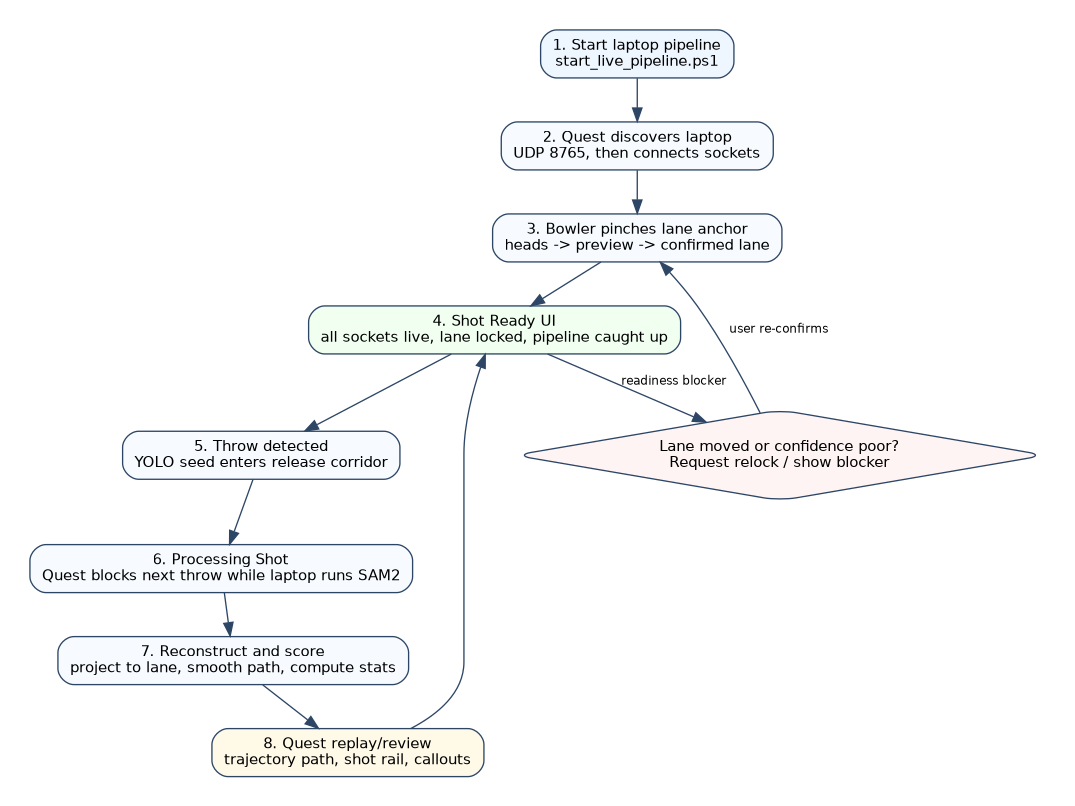
\includegraphics[width=0.92\textwidth]{original_04_clean_padded.png}
  \caption{End-to-end interaction flow reconstructed from the Quest UI state graph and laptop pipeline.}
\end{figure}

\begin{figure}[ht]
  \centering
  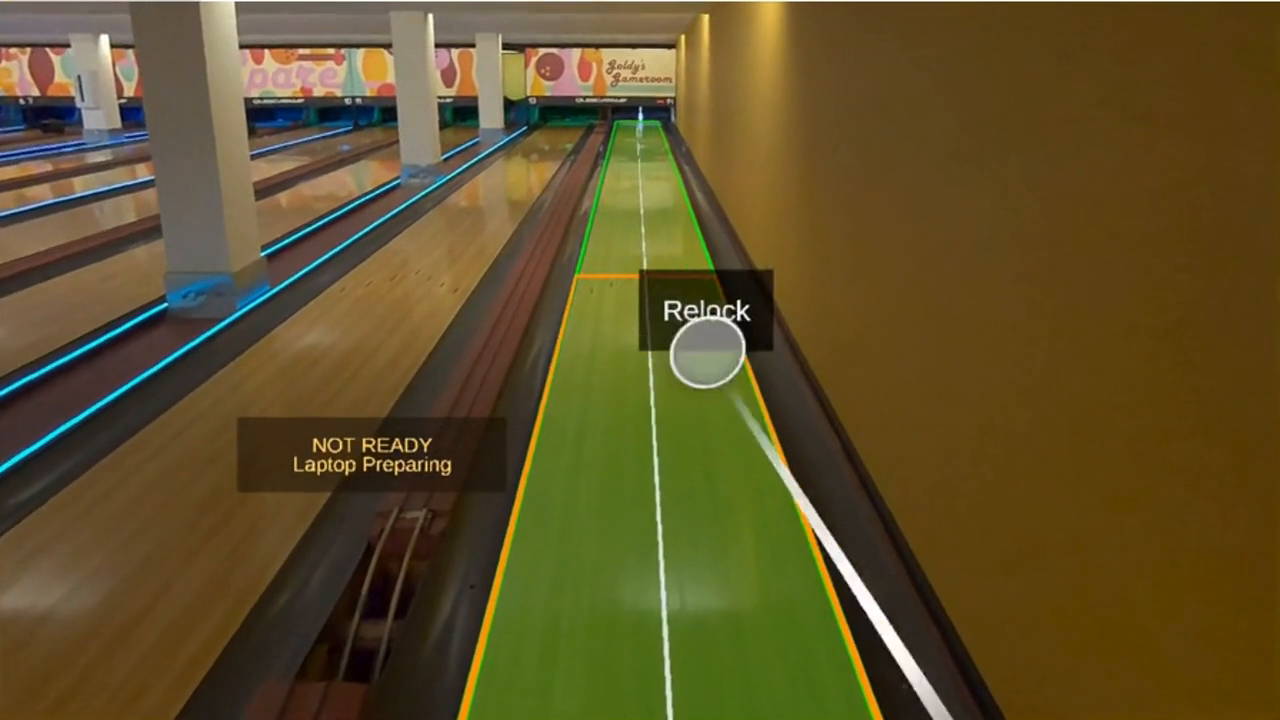
\includegraphics[width=0.62\textwidth]{lane_lock_relock_process_final.png}
  \caption{Lane-lock detail: the bowler confirms the aligned overlay before the laptop can use the lane geometry for detection and replay.}
\end{figure}

This flow changed substantially during development. Early prototypes were good at showing isolated pieces, but the live product needed strong session state. We learned that the headset should not show lane placement while the laptop is disconnected, nor should it show \emph{Shot Ready} just because the lane is confirmed. The final state graph resolves the first blocking reason and uses clear labels such as \emph{Laptop Connecting}, \emph{Media Stream Not Ready}, \emph{Results Reconnecting}, \emph{Pinch + Hold Lane}, \emph{Confirm Lane}, \emph{Laptop Catching Up}, and \emph{Processing Shot}. This makes the user interface a reflection of the actual runtime, not a separate optimistic display.

\section{Implementation}

\begin{figure}[t]
  \centering
  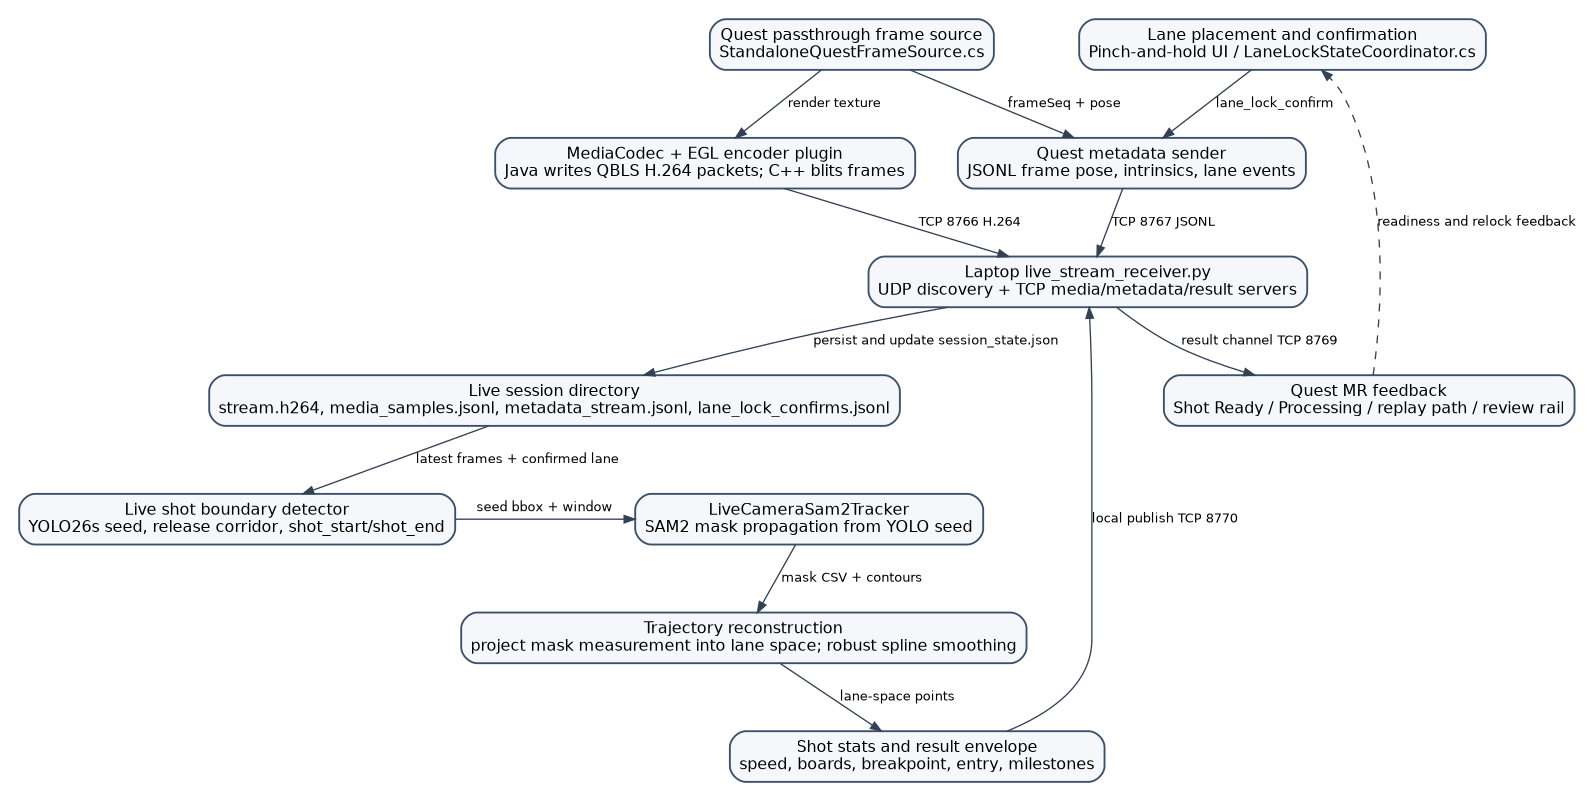
\includegraphics[width=0.94\textwidth]{original_06.png}
  \caption{System architecture: Quest capture and lane lock, media and metadata streams, laptop analysis pipeline, and result return path.}
\end{figure}

\begin{figure}[t]
  \centering
  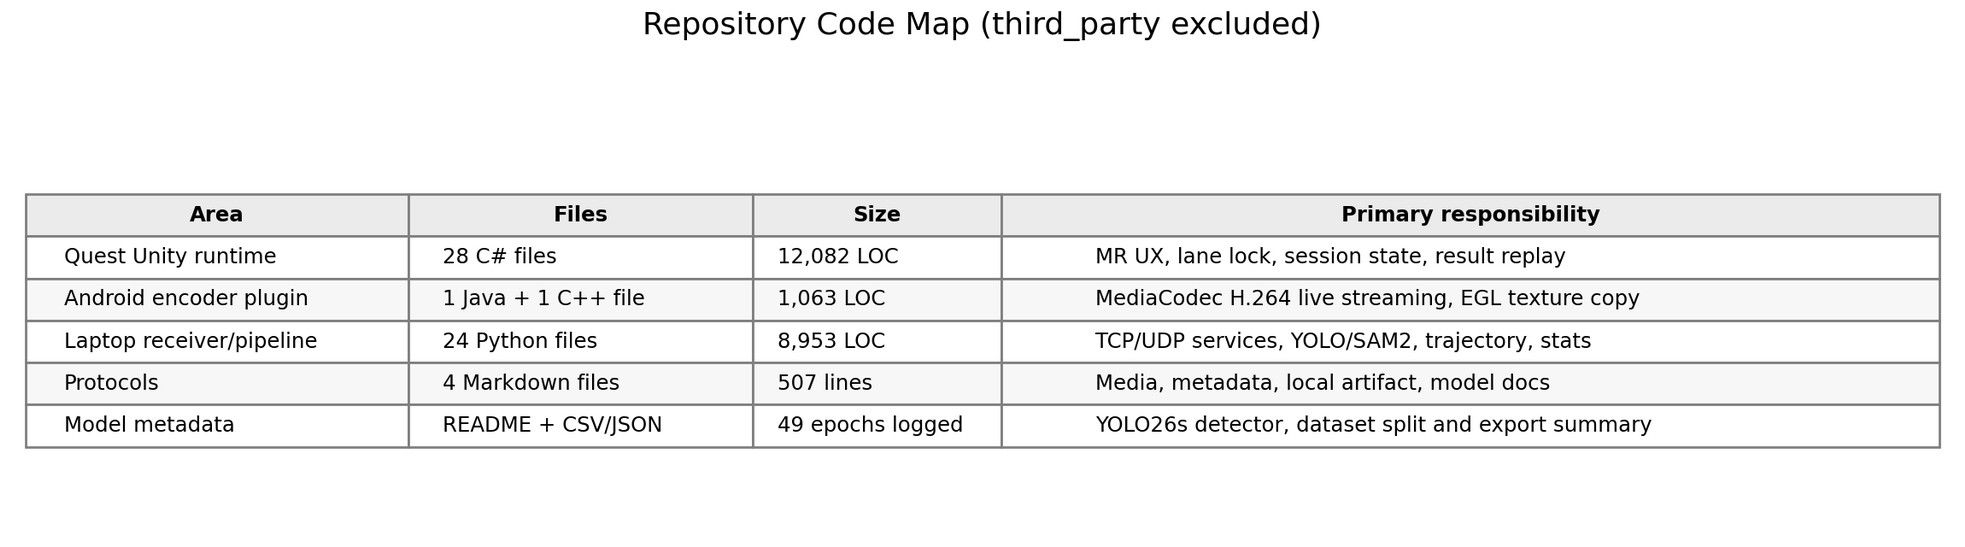
\includegraphics[width=0.92\textwidth]{original_03.jpeg}
  \caption{Repository code map showing major implementation areas and responsibility boundaries.}
\end{figure}

\subsection{Quest Runtime}

The Quest implementation lives in \texttt{unity\_proof/Assets/StandaloneProof}. It is a Unity application built for Quest 3. The key runtime components are the session controller, lane lock coordinator, metadata sender, result receiver, state graph, replay renderer, and review UI.

The session controller manages laptop discovery and the live session lifecycle. It opens the H.264 media stream, metadata stream, and result stream, and it keeps the application from presenting an invalid \emph{Shot Ready} state. The metadata sender emits session start, frame metadata, lane lock confirmation, shot boundary, and session end records. The result receiver listens for laptop messages and marshals pipeline status and shot results back onto Unity's main thread.

The lane lock coordinator owns the bowler interaction for lane placement. The user must place, preview, and confirm the lane. Once confirmed, the Quest sends the actual lane geometry to the laptop rather than asking the laptop to infer lane geometry from arbitrary frames. This became important after field testing showed that small calibration errors were amplified down the 60 ft lane.

The replay renderer validates results before drawing them. It expects the current trajectory point definition, checks that the result belongs to the current lane lock request, and rejects low-confidence or mostly off-lane trajectories. This prevents delayed or stale laptop results from drawing in the wrong coordinate frame.

\subsection{H.264 Streaming and Protocol}

The Android encoder plugin avoids CPU readback by sending Unity textures into Android MediaCodec. The plugin writes encoded samples into a live TCP media stream while the metadata channel remains JSONL. The binary media protocol uses a small header with magic bytes, version, packet type, and payload length. JSON channels are human-readable, which made field debugging practical.

\begin{table}[t]
  \centering
  \begin{tabular}{@{}lll@{}}
    \toprule
    Channel & Port & Purpose \\
    \midrule
    UDP & 8765 & Laptop discovery \\
    TCP & 8766 & H.264 media stream \\
    TCP & 8767 & Frame metadata and lane confirmations \\
    HTTP & 8768 & Receiver health \\
    TCP & 8769 & Laptop-to-Quest results \\
    TCP & 8770 & Local result publish into receiver \\
    \bottomrule
  \end{tabular}
  \caption{Final live runtime ports.}
\end{table}

The laptop receiver stores the full session in one \codepath{data/incoming_live_streams/} session directory. Important files include \codepath{stream.h264}, \codepath{media_samples.jsonl}, \codepath{metadata_stream.jsonl}, \codepath{lane_lock_confirms.jsonl}, \codepath{shot_boundaries.jsonl}, \codepath{analysis_camera_sam2/}, \codepath{analysis_live_shots/}, \codepath{outbound_results.jsonl}, and \codepath{session_state.json}. This persistent session directory turned out to be one of the most useful engineering choices: every live failure could be replayed and inspected after leaving the bowling alley.

\subsection{Laptop Vision Pipeline}

The laptop pipeline uses YOLO and SAM2 for different jobs. YOLO is responsible for causal discovery of the bowling ball. It scans decoded H.264 frames and finds the first high-confidence, lane-valid seed. SAM2 is then responsible for mask tracking across the live shot window. This division is more reliable than asking YOLO to redetect the ball on every frame, and faster than waiting for SAM2's default offline video predictor to initialize on a completed clip.

\begin{figure}[t]
  \centering
  \begin{subfigure}{0.48\textwidth}
    \centering
    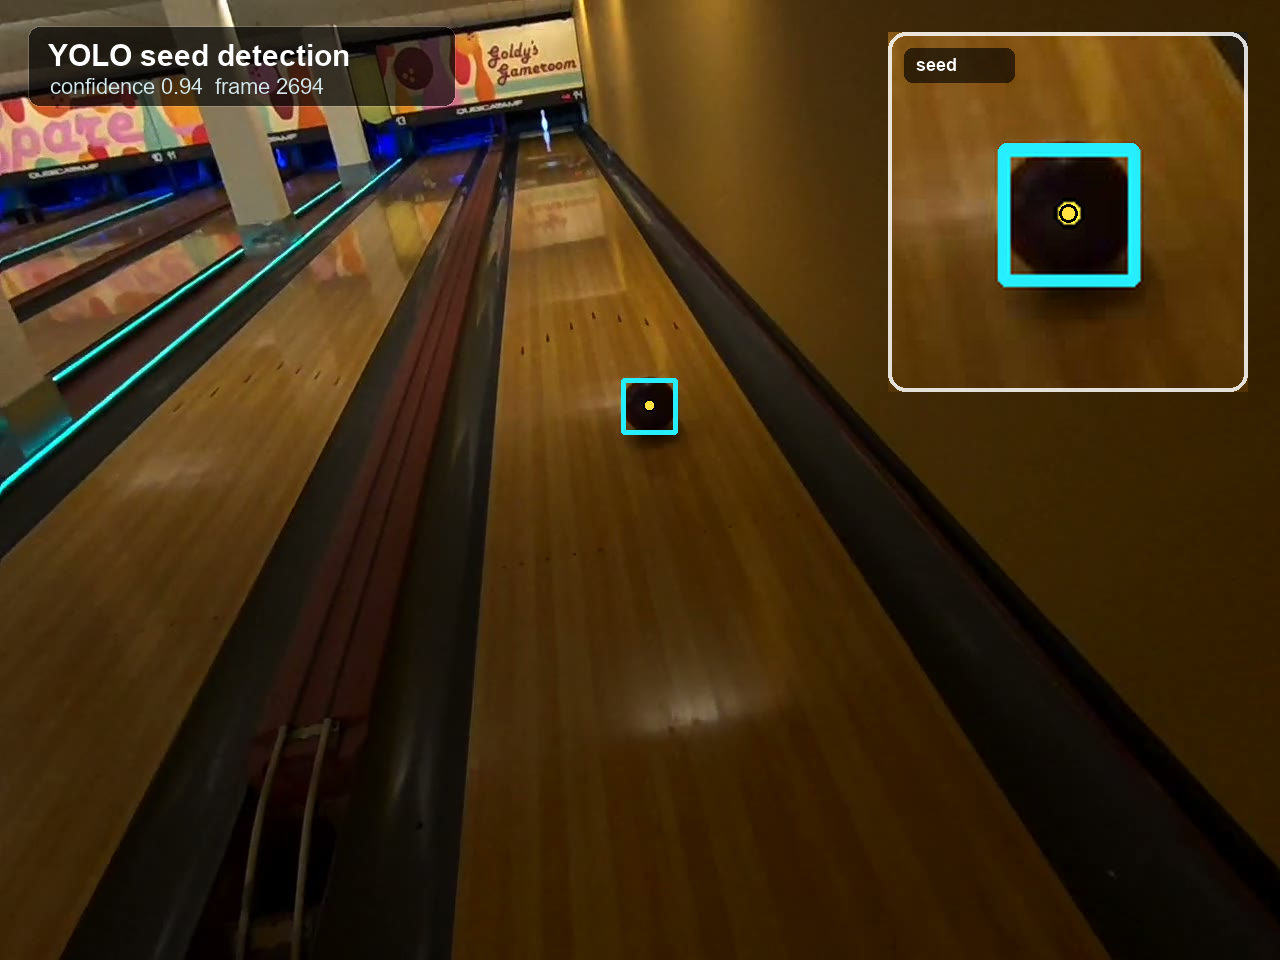
\includegraphics[width=\linewidth]{yolo_seed_detection_frame.png}
    \caption{YOLO supplies the first reliable ball seed and must pass lane/release-corridor checks.}
  \end{subfigure}
  \hfill
  \begin{subfigure}{0.48\textwidth}
    \centering
    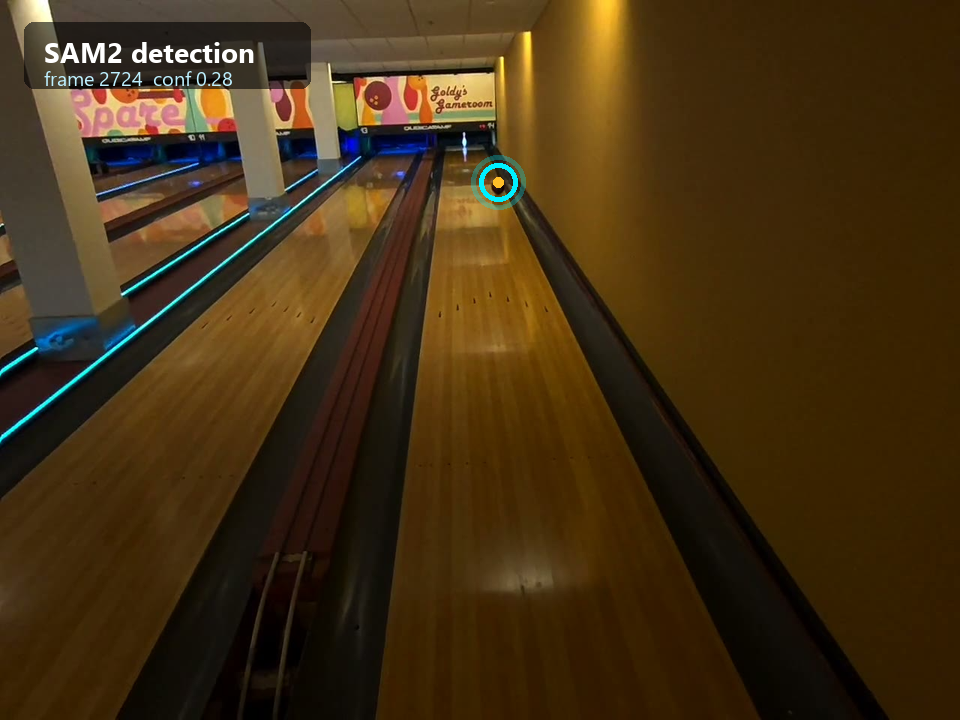
\includegraphics[width=\linewidth]{sam2_detection_frame.png}
    \caption{SAM2 tracks the ball mask through the live shot window.}
  \end{subfigure}
  \caption{The live detector uses YOLO for causal seeding and SAM2 for frame-by-frame mask tracking.}
\end{figure}

The project uses SAM2's camera predictor path rather than the default completed-video predictor path. The camera predictor allows the code to call \texttt{load\_first\_frame(...)} on the YOLO seed frame and then \texttt{track(frame)} as decoded frames arrive. The model is loaded and warmed once, then reused across shots. This was a major latency improvement because the system no longer waits for a full clip before beginning tracking.

Shot detection also required runtime tuning. The detector scans with a stride, checks projection confidence, verifies that the ball is inside the release corridor, and confirms downlane motion before opening a shot. During field testing, backlog handling became important: if the laptop fell behind, the UI showed \emph{Laptop Catching Up} and the detector could fast-forward near the current live point before rearming. This reduced the chance of throwing while YOLO was still processing old frames.

\subsection{Geometry, Trajectory Reconstruction, and Statistics}

The lane lock result defines the lane coordinate system. The laptop reconstructs camera rays from image coordinates and camera intrinsics, intersects those rays with the locked lane plane, and converts the intersection into lane coordinates. The final trajectory point definition is \texttt{camera\_sam2\_mask\_measurement\_spline\_l14}, reflecting that the point comes from a SAM2 mask measurement and robust lane-space spline smoothing.

The project originally experimented with Kalman filtering, but field plots showed that an overly physical smoother could underrepresent real hook shape or create misleading behavior at the end of the lane. The final approach uses lane-space smoothing with a fixed lambda chosen from the recorded six-shot session. This keeps the replay visually stable without pretending that far-lane observations are as reliable as near-lane observations.

The statistics module computes bowling-focused metrics: speed, speed loss, board at arrows, breakpoint, entry board, entry angle, and related milestones. Speed is reported in mph. For reliability, downlane speed is computed from downlane distance rather than noisy 2D path length. Gutter or edge cases are also treated carefully; not every metric makes sense for every shot.

\begin{center}
  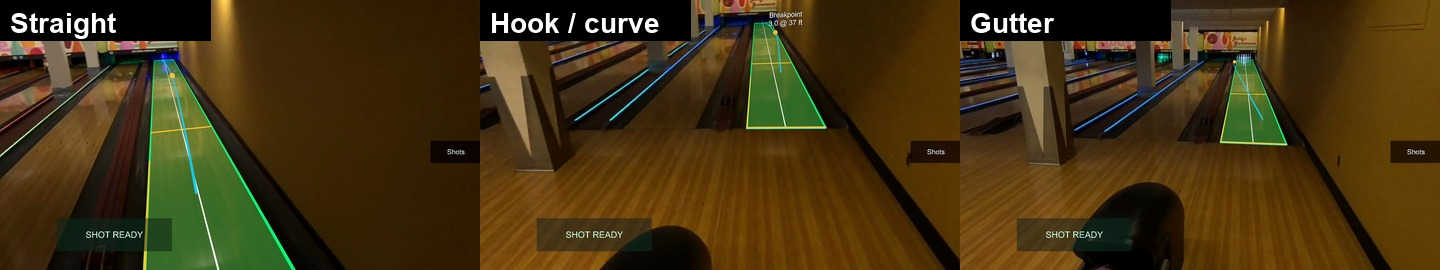
\includegraphics[width=0.78\textwidth]{trajectory_three_shots_selected_contact.jpg}
  \captionof{figure}{Field-trial outputs showing a straighter shot, a hook shot, and an edge/gutter case reconstructed by the same live pipeline.}
\end{center}

\section{Model and Dataset Decisions}

The bowling-ball detector was trained specifically for this project. We considered YOLO11 and YOLO26 variants and selected YOLO26s because it offered a modern architecture at roughly the small-model parameter budget. The training notes identify YOLO26s as a useful upgrade over YOLO11s because of its newer detection design, better small-object behavior, and strong deployment fit.

The dataset work was intentionally efficient. Instead of manually labeling every frame, we manually curated 40 accepted bowling runs across two alleys and used SAM-assisted exports to create 641 positive images and 160 negative images. That meant roughly 40 manually reviewed clips turned into about 810 training images. The split was run-based rather than frame-random: 34 runs for train, 3 for validation, and 3 for test. A run-based split is important because adjacent video frames are highly correlated; a random frame split would exaggerate performance.

\begin{figure}[ht]
  \centering
  \begin{subfigure}{0.48\textwidth}
    \centering
    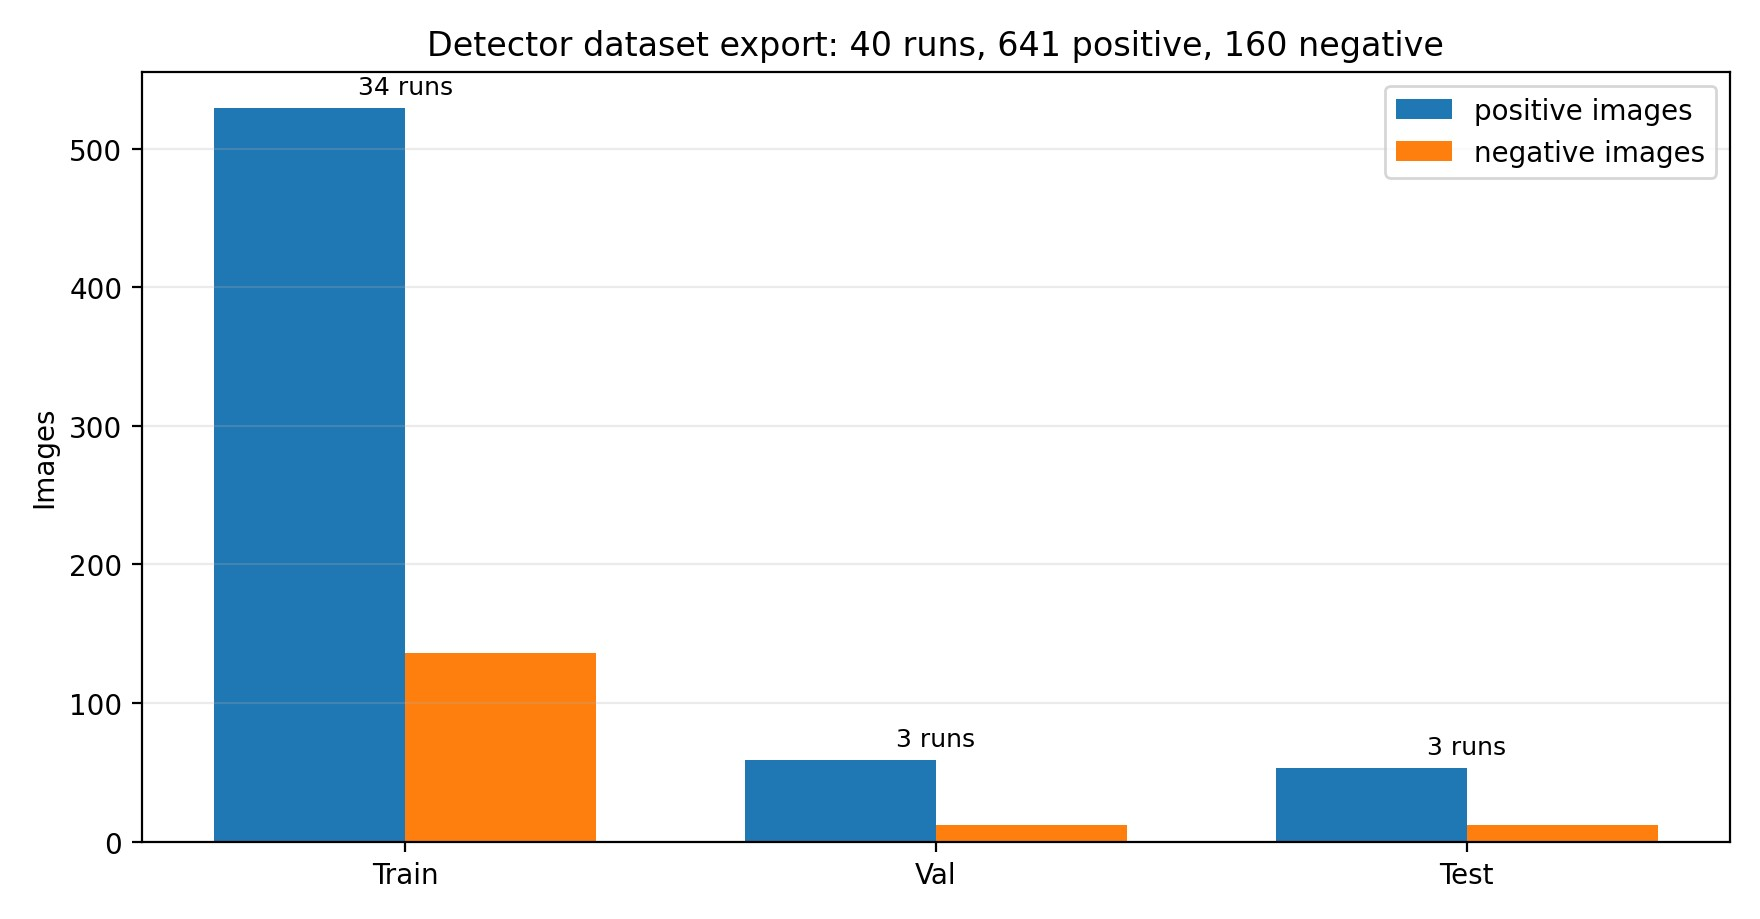
\includegraphics[width=\linewidth]{original_01.jpeg}
    \caption{Run-based dataset split after SAM-assisted export.}
  \end{subfigure}
  \hfill
  \begin{subfigure}{0.48\textwidth}
    \centering
    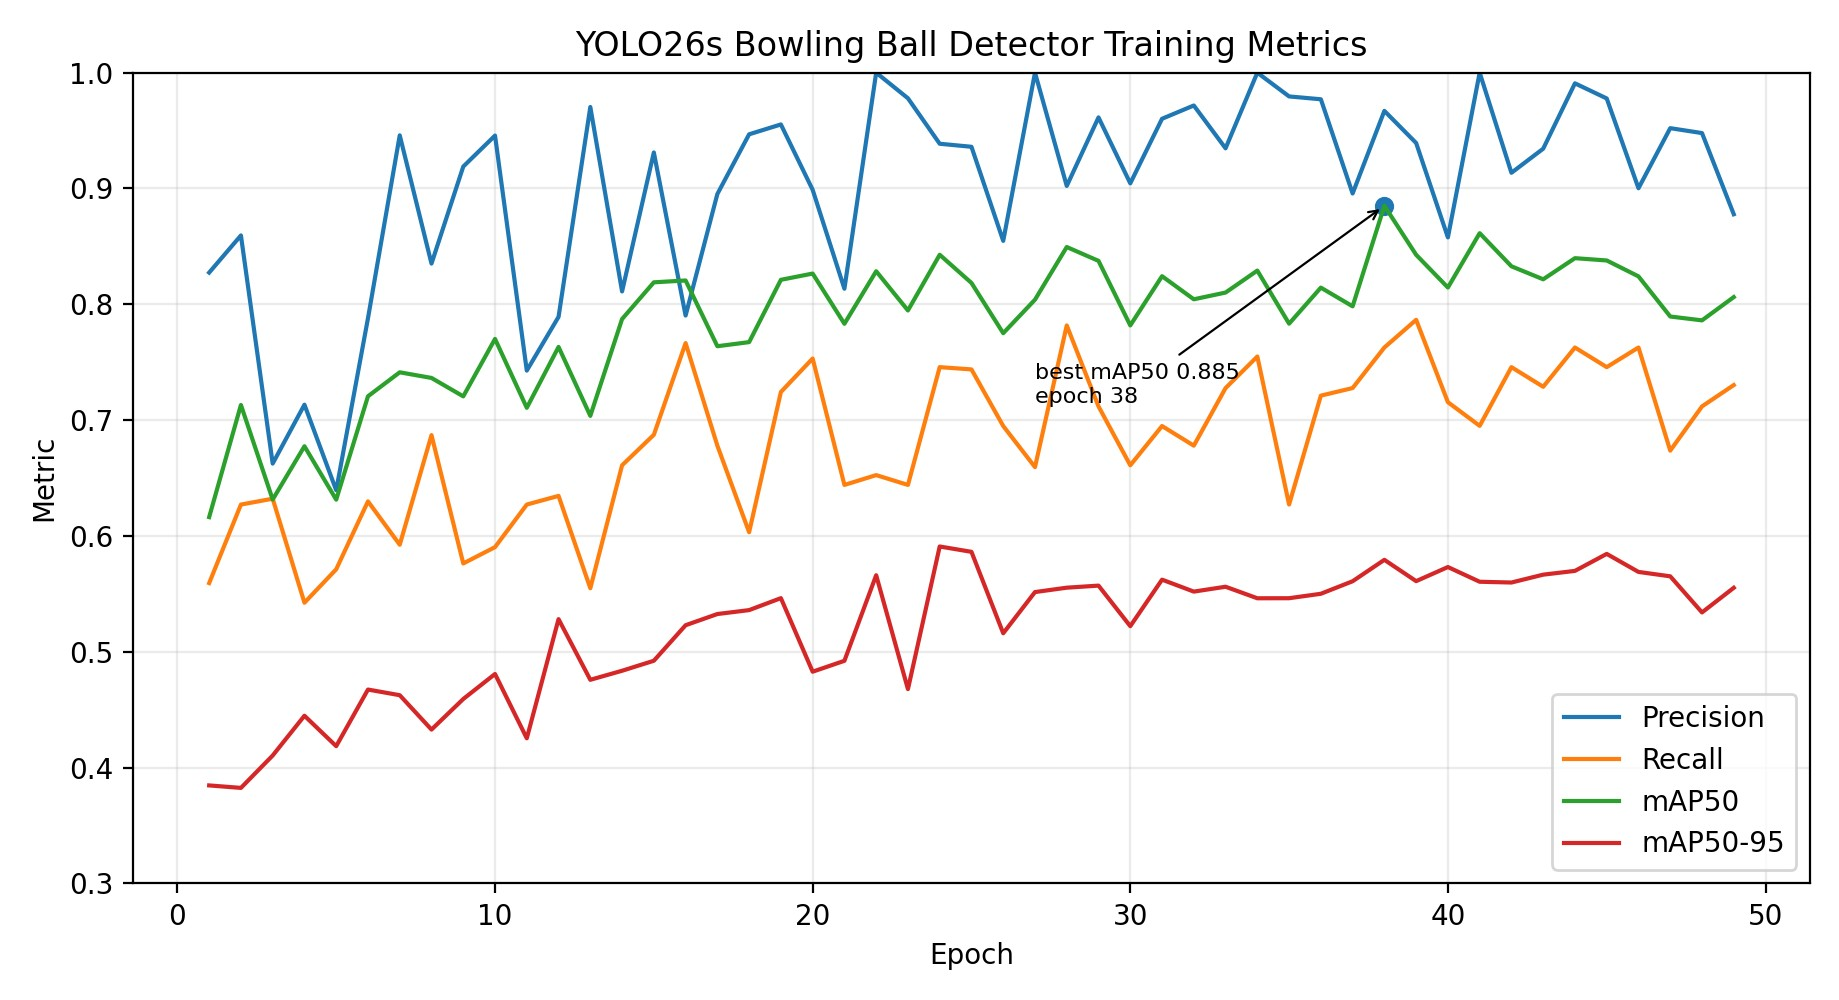
\includegraphics[width=\linewidth]{original_02.jpeg}
    \caption{YOLO26s training curves from the repository results file.}
  \end{subfigure}
  \caption{Detector dataset and training evidence used to choose the final YOLO26s checkpoint.}
\end{figure}

\begin{center}
  \begin{tabular}{@{}ll@{}}
    \toprule
    Item & Value \\
    \midrule
    Detector & YOLO26s \\
    Training runs & 34 \\
    Validation runs & 3 \\
    Test runs & 3 \\
    Positive images & 641 \\
    Negative images & 160 \\
    Held-out test mAP50 & 0.839 \\
    Test precision & 0.974 \\
    Test recall & 0.721 \\
    \bottomrule
  \end{tabular}
  \captionof{table}{Summary of detector data and held-out performance.}
\end{center}

The final held-out Alley B test set reported mAP50 around 0.839, precision around 0.974, and recall around 0.721. For this system, high precision is more important than maximum recall. A missed ambiguous seed delays or skips a replay, but a false seed can cause SAM2 to track the wrong object and produce a misleading trajectory.

We also published the YOLO training dataset on Hugging Face so the dataset can be reused as an open-source contribution. The dataset contains bowling-ball images and YOLO labels; it does not intentionally label people or faces. The project README links to the dataset and documents the expected runtime checkpoint path.

\section{User Interface and Demo Design}

The Quest UI changed significantly near the end of the project. Early versions allowed too many controls or showed stale replay UI during throw preparation. The final design uses a simple principle: while the bowler is preparing to throw, the center of the view should stay quiet. \emph{Shot Ready} is the primary signal. Review and shot rail elements should not block the lane during the throw.

The final demo video was built in Remotion so that video, stills, generated narration, and labels could be placed deterministically. The video is about 2 minutes and 14 seconds. It explains the motivation, lane setup, YOLO/SAM2 pipeline, field trials, session review, the far-lane tracking limitation, and final closing notes. OpenAI text-to-speech was used for narration so the demo did not require manual voice-over recording.

\section{Evaluation}

Our evaluation was limited and mostly technical rather than a formal user study. Because the project required a bowling alley, a Quest headset, a laptop GPU, and a stable live network setup, we spent most of the evaluation time on field trials and end-to-end debugging. We did not complete a structured three-participant external study, so the results below should be read as prototype validation rather than conclusive usability evidence.

The most important evaluation was whether the system could run through the full loop in the field: place the lane, stream Quest passthrough video to the laptop, detect the bowling ball with YOLO, initialize SAM2 tracking, reconstruct the lane-space trajectory, compute stats, publish the result, and replay it in the headset. By the final field session, we captured a six-shot recording with successful examples of straight shots, hook shots, and a gutter shot. These runs showed that the pipeline can produce useful replays when the lane calibration is stable and the ball is visible through the early and middle lane.

We also evaluated the system through logged runtime metrics. Earlier versions had replay delays that grew across shots because the detector could fall behind the H.264 stream. After changing the detector to keep a hot sequential decoder and after adding backlog recovery, later shots no longer required expensive re-decoding from the start of the session. We also used per-shot diagnostics to verify when YOLO ran, when SAM2 started, how many frames were processed, and when results were published back to Quest.

The clearest negative result was far-lane tracking. Around the 45--60 ft region, the ball becomes very small in the camera image. In our recorded six-shot session, the SAM2 mask radius near that range was about 9 px, and a one-pixel mask shift could project to roughly 0.60 ft or 0.72 boards in lane space. This explains why early and mid-lane trajectory feedback is more trustworthy than pin-deck entry statistics. That limitation is included in the final demo instead of being hidden.

From a usability perspective, our own field use revealed several issues that were fixed before the final version: stale replay overlays blocking the next throw, readiness labels that appeared before the laptop was actually connected, cluttered trajectory callouts, and lane-lock controls sitting too close to the center of the bowling view. These were not formal user-study findings, but they were real issues observed during repeated live use of the prototype.

The main evaluation takeaway is that the end-to-end concept works, but the current evidence is still prototype-level. A stronger follow-up evaluation would recruit bowlers, compare replay stats against a commercial lane system or manual video annotation, and measure whether the feedback actually helps users adjust their next shot.

\section{Reflection}

The project began as a computer-vision idea, but the hardest work was synchronization. A live MR sports system fails if the camera frame, pose, lane lock, model output, trajectory, and headset overlay do not agree. Much of the final engineering effort went into making that chain explicit through stable session directories, schema contracts, lane lock IDs, result envelopes, readiness gates, and replay validation.

Work was split across the team in complementary streams. Cale Rudolph focused on MR interaction, UI, and trial/demo capture. Srinivas Kantha Reddy focused on Quest streaming, YOLO/SAM integration, and end-to-end runtime debugging. Apurv Kushwaha focused on the laptop computer-vision pipeline, lane segmentation/calibration work, and trajectory reconstruction support. All team members contributed to field testing, debugging, final presentation work, and final demo assets.

In hindsight, we would define the protocol and state machine earlier. We spent time fixing issues that came from hidden state: stale media streams, optimistic UI readiness, lane calibration mismatch, and result delivery. We would also collect more controlled evaluation data earlier, especially across different alleys and lighting conditions.

The most important technical lesson was that reliable capture and logging come before model quality. YOLO and SAM2 worked offline before the live product felt dependable. The product became useful only after we could answer, for every shot, which frames were processed, which lane lock was used, when the result was computed, and why the headset did or did not show \emph{Shot Ready}.

\section{Limitations and Future Work}

The main limitation is the final 15 ft of the lane. In our six-shot session, the ball mask radius dropped to about 9 px in the 45--60 ft range. At that distance, one pixel of SAM2 mask drift can project to roughly 0.60 ft and 0.72 boards, so a few pixels can become a visible trajectory or entry-board error. Near-lane and mid-lane measurements are more reliable than pin-deck statistics.

Other limitations include lighting variation, reflections, occlusion near gutters and pins, accurate lane calibration, and dependency on a laptop GPU for SAM2. The current system also requires setup steps: laptop hotspot, pipeline process, Quest install, and proximity-sleep handling.

Future work includes improving far-lane tracking, integrating scoring data, adding richer session export, supporting coach review workflows, and visualizing confidence by fading low-confidence far-lane extrapolations.

\enlargethispage{4\baselineskip}
\section{Acknowledgments and References}

We acknowledge the tools and resources that made the project possible: Meta Quest 3 passthrough APIs, Unity, Android MediaCodec, OpenCV, Python, PyTorch, Ultralytics YOLO, and Meta SAM2. We also thank the instructor and classmates for feedback, and Goldy's Gameroom for field testing space.

\begin{itemize}[itemsep=0.15em,topsep=0.25em]
  \item \reportlink{https://github.com/sri299792458/QuestBowlingStandalone}{QuestBowlingStandalone repository}
  \item \reportlink{https://huggingface.co/datasets/sri299792458/quest-bowling-ball-yolo}{Published YOLO dataset}
  \item \reportlink{https://drive.google.com/file/d/1ChvX2wGKDNvMor3lKa0ZUYFAq08_IGWq/view}{Final demo video}
\end{itemize}
\end{document}
